\subsection{Étude de la variable species}

\vspace{.2cm}

\noindent
\textbf{Question~5~:} Quels sont les effectifs de chaque modalité~? 
\vspace{.2cm}

Le code \textit{Python} suivant permet de calculer l'effectif de chaque espèce, soit les modalités de la variable qualitative \textit{class}. 
On trouve qu'au final il y a 50~Iris de chaque espèce.
\begin{lstlisting}[style=myPython, caption=Code Pyton pour déterminer les effectifs de chaque modalités, frame=lines]
for spe in species:
    if spe == 'Iris-setosa':
        iris_setosa += 1
    elif spe == 'Iris-versicolor':
        iris_versicolor += 1
    elif spe == 'Iris-virginica':
        iris_virginica += 1

print("effectif de la modalité iris_setosa", iris_setosa)
print("effectif de la modalité iris_versicolor", iris_versicolor)
print("effectif de la modalité iris_virginica", iris_virginica)
\end{lstlisting}

\begin{lstlisting}[style=myLog, caption=Résultat du code, frame=lines]
effectif de la modalité iris_setosa 50
effectif de la modalité iris_versicolor 50
effectif de la modalité iris_virginica 50
\end{lstlisting}

\vspace{.5cm}


\noindent
\textbf{Question~6~:} Les représentations graphiques classiques liées aux variables qualitatives sont la 
représentation en secteurs ou camembert (pie), la représentation en bâtons (hist). Représenter ces graphiques. (pour Python vous pouvez utiliser matplotlib.pyplot)
\vspace{.2cm}

\begin{figure}[!h]
    \centering
    \begin{minipage}{.48\linewidth}
        \begin{center}
            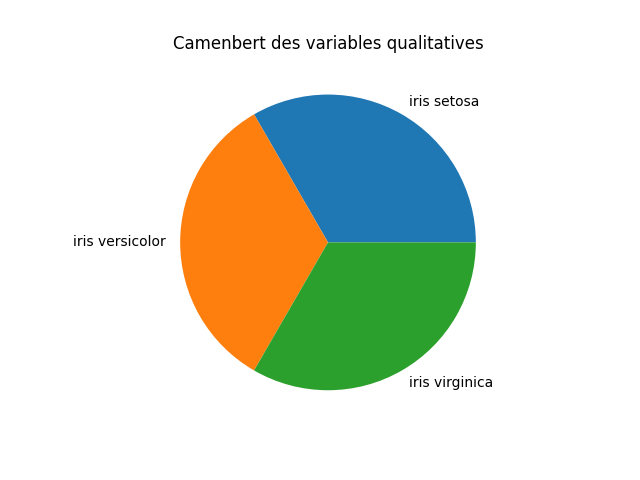
\includegraphics[width=1.1\textwidth]{img/Figure_1.png}
            \caption{\label{fig:camembert}Diagramme camembert des variables qualitatives}  
    \end{center}
    \end{minipage}\hfill
    \begin{minipage}{.48\linewidth}
        \begin{center}
                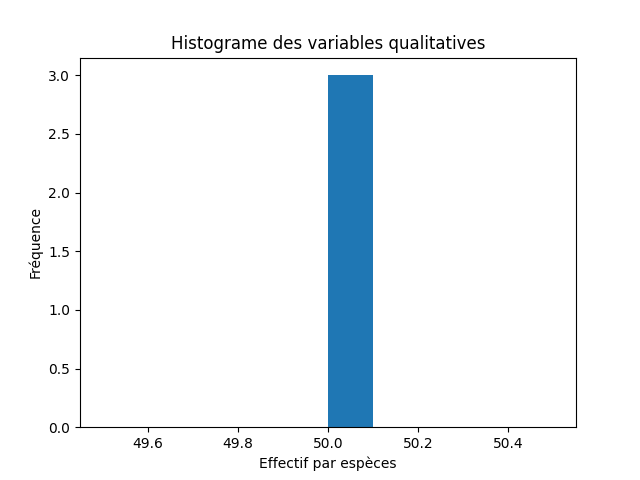
\includegraphics[width=1.1\textwidth]{img/Figure_2.png}
                \caption{\label{fig:histogramme_var-qualitatives}Histogramme des variables qualitatives}  
        \end{center}
    \end{minipage}
\end{figure}

\begin{lstlisting}[style=myPython, caption=Code Python pour tracer le diagramme camenbert et l'histogramme, frame=lines]
nb_species = np.array([iris_setosa, iris_versicolor, iris_virginica])
plt.pie(nb_species, labels=["iris setosa", "iris versicolor", "iris virginica"])
plt.title("Camenbert des variables qualitatives")
plt.show()

plt.hist(nb_species)
plt.title("Histograme des variables qualitatives")
plt.show()
\end{lstlisting}

